\subsection{Alpha Decay}
\begin{itemize}
    \item As seen in \cref{fig: radioactive_nuclei_chart}, heavier nuclei tend to decay by emitting an $\alpha$ particles, and are often referred to as $α$ emitters. 
    \item This is caused by the Coulomb force having a much longer range than the strong force. As nuclei grows large, they need more neutrons to stabilize the nucleus, but it can quickly become too much. 
    \item $α$ particles are the most tightly bound, and calculated to be the only way to decay with a positive Q-value, making it spontaneous. One could imagine just emitting a single proton, but the Q-value would be negative.
    \begin{equation}
      \ce{_{}^{232}\text{U}_{}} → \ce{_{}^{4}\text{He}_{}} + \ce{_{}^{228}\text{Th}_{}}
    \end{equation}
    \begin{equation}
      Q_{α} = M\left(\ce{_{}^{232}\text{U}_{}}\right) - \Big(M\left(\ce{_{}^{4}\text{He}_{}}\right) + M\left(\ce{_{}^{228}\text{Th}_{}}\right)\Big)c^2 = 5.41 \text{ MeV}
    \end{equation}
\end{itemize}

\subsubsection{Energetics of Alpha Decay}
We take the general case of:
\begin{equation}
  \ce{_{Z}^{A}\text{X}_{N}} → \ce{_{Z-2}^{A-4}\text{Y}_{N-2}} + α
\end{equation}
The we have energy conservation, where $T$ is the kinetic energy and $p$ is the momentum:
\begin{equation}
  m_{X}c^2 = m_{Y}c^2 + T_{Y} + m_{α}c^2 + T_{α}
\end{equation}
\begin{equation}
  \Big(\underbrace{m_{X} - \left(m_{Y} + m_{α}\right)}_{Q-\text{value}}\Big)c^2 = T_{Y} + T_{α}
\end{equation}
\begin{equation}
  Q = T_{Y} + T_{α}
\end{equation} 
As we assume the system is at rest, there should be no net momentum. We do not care about the sign. 
\begin{equation}
  p_{Y} = p_{α}   
\end{equation}
We get the kinetic energy of the $\alpha$ particle:
\begin{equation}
  T_{α} = \frac{Q}{1 + m_{α}/m_{Y}}
\end{equation}

This resembles the taylor expansion of $1/(1 + x)$:
\begin{equation}
  \frac{1}{1 + x} = 1 - x + x^2 - x^3 + \dots
\end{equation}
From this we get an approximation for the kinetic energy of the $\alpha$ particle from the Q-value. As it is easy to measure the momentum of the $α$ particle, we have a shortcut to the Q-value.
\begin{equation}
  T_{α} = Q\left(1 - \frac{m_{α}}{m_{Y}}\right) = Q\left(1 - \frac{4}{A}\right)\quad , \quad  m_{α} ≈ 4 \ , \ m_{Y} ≈ A
\end{equation}


\subsubsection{$Q$-value and Half-life}
\begin{itemize}
  \item The $Q$-value is closely related to the half-life of the decay.
  \item The greater the $Q$-value, the shorter the half-life. This makes sense as it is very energetically favorable to decay.
  \item Even-odd and odd-even $α$ emitters have a 2-1000 times greater periods than even-even emitters. Even when $Z$ and $Q$ are the same. 
\end{itemize}

\subsubsection{$Q$ vs $A$ Systematics (\cref{fig: Q_v_A_systematics})}
\begin{figure}[h!]
\centering
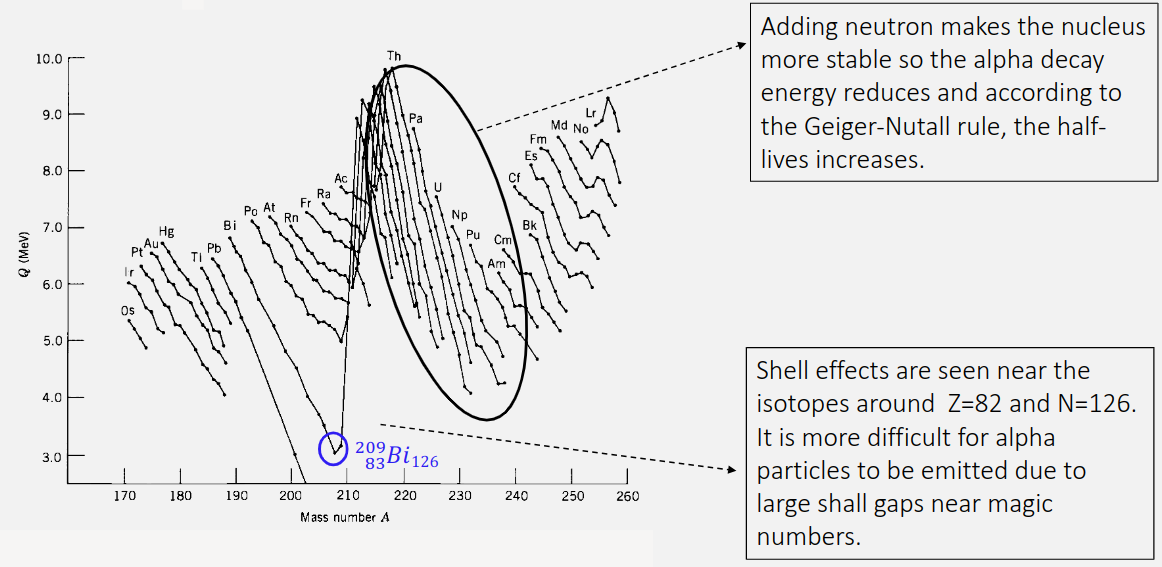
\includegraphics[width = .8\textwidth]{Q_v_A_systematics.png}
\caption{}
\label{fig: Q_v_A_systematics}
\end{figure}

\subsubsection{Theory of Alpha Decay}
\begin{itemize}
  \item Assuming the nucleus is full of alpha particles, we can calculate the probability of the alpha particle quantum tunneling through the potential barrier of the nucleus.
  \item We can view the regions as seen in \cref{fig: alpha_square_well} described classically or quantum mechanically.
\end{itemize}

\parbox[t]{\dimexpr\textwidth-\leftmargin}{%
\paragraph{Classical View}
\begin{wrapfigure}{r}{0.45\textwidth}
\vspace{3mm}
\centering
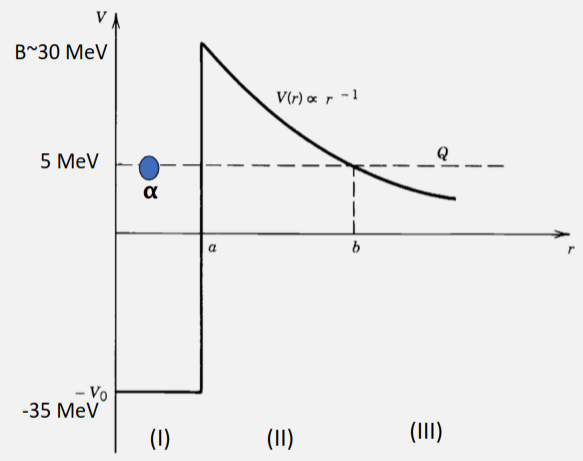
\includegraphics[width = .4\textwidth]{alpha_square_well.png}
\caption{Simple model of the nuclear potential creating a square well for the alpha particle. }
\label{fig: alpha_square_well}
\end{wrapfigure}
\begin{enumerate}[(I)]
  \item The alpha particle moves inside the potential well, but can't escape. 
  \item The region of the potential well. The alpha particle can't enter this region, as the potential is too high.
  \item Classically, the alpha particle is permitted to be on the outside, in this region, as the potential is lower than the energy of the alpha particle.
\end{enumerate}
\vspace{5mm}
}
  
  
\paragraph{Quantum Mechanical View}
\begin{itemize}
  \item The alpha particle will try to penetrate the potential barrier, and will make it after many attempts. 
  \item The barrier delays the emission. This is what gives the long half-life of alpha emitters. 
  \item The probability $λ$ of decay depends on frequency (how often the alpha particle tries to penetrate the barrier) and the probability of success. For alpha waves we have $λ = fP$. 
\end{itemize}

\paragraph{Example: $\ce{_{}^{235}\text{U}_{}}$}
\begin{itemize}
  \item We can calculate the barrier height $B$, by assuming we have an alpha particle stuck inside a thorium nucleus (as $\ce{_{92}^{235}\text{U}_{}} → \ce{_{90}^{231}\text{Th}_{}} + \ce{_{}^{4}\text{He}_{}}$). We inserting the number of protons in the Helium $Z_1$ and Thorium $Z_2$, and the radius of the two nuclei $R_1$ and $R_2$ into the formula. The radius is found by $R = R_0A^{1/3}$, where $R_0 = 1.2$ fm.
  \begin{equation}
    B = \frac{e^2}{4πϵ_0} \frac{Z_1 Z_2}{R_1 + R_2} = 1.44 \text{ MeV} ⋅  \text{fm} ⋅ \frac{2 ⋅ 90}{1.2 \left(4^{1/3} + 231^{1/3}\right)} ≈ 28 \text{ Mev}
  \end{equation}
  
  \item The Q-decay energy of the alpha particle is $4.6$ Mev. 

  \item The velocity of the alpha particle is found through the kinetic energy. The kinetic energy 
  \begin{equation}
    E_k = 5 + 35  = 40\text{ Mev} → v = 4.5 ⋅ 10^{7} \text{ m/s}
  \end{equation}
  \item The time it takes the particle to travel to the barrier can then be found:
  \begin{equation}
    t = R/v = \frac{7.5 ⋅ 10^{15}m}{4.5 ⋅ 10^{7}m/s} = 1.67 ⋅ 10^{-21}s
  \end{equation} 
  \item The frequency of the alpha particle trying to penetrate the barrier is then $f = 1/t = 6 ⋅ 10^{21}s^{-1}$.
  \item As the half-life of Uranium is around $10^9$, the alpha particle will attempt to penetrate the barrier $10^{41}$ times.
\end{itemize}

\subsubsection{Spin and Parity in Alpha Decay}
The total angular momentum carried by the alpha particle is only orbital, meaning $j_{α} = l_{α}$. The possible values of a final state $J_f$, from an initial state $J_i$ is given by $\left|J_i - J_f\right| ≤ l_{α} ≤ J_i + J_f$, with parity $π = (-1)^{l_α}$.

\paragraph{Example:}
\begin{wrapfigure}[9]{r}{0.5\textwidth}
\vspace{-5mm}
\centering
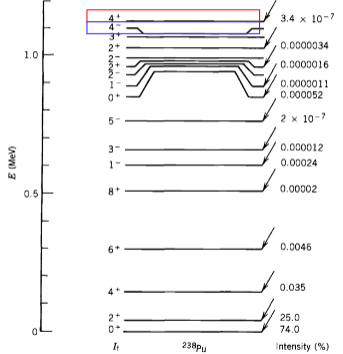
\includegraphics[width = .45\textwidth]{decay_intensity_by_state.png}
\caption{decay intensity of $\ce{_{}^{242}\text{Cm}_{}}$ to different excited states of $\ce{_{}^{238}\text{Pu}_{}}$. Blue: $4^{-}$-state, Red: $4^{+}$-state}
\label{fig: decay_intensity_by_state}
\end{wrapfigure}


Using the parity of each state as shown in \cref{fig: decay_intensity_by_state}, we can determine if a decay is allowed. As seen in blue, the $4^{-}$-state has $l_{α} = 4$, giving positive parity. This is conserved and therefore allowed. As seen in blue, we have the opposite, with non-conserved parity, which is therefore not allowed. 

If $l_{α}$ is even, the parity must be positive, and if $l_{α}$ is odd, the parity must be negative.

\vspace{40mm}